Trace la gráfica de un ejemplo de una función $f$ que cumpla con todas las condiciones dadas.

\begin{enumerate}[label=\alph*)]
  \item $\ds\lim _{x \rightarrow-4^{+}} f(x)=-\infty$
  \item $\ds\lim _{x \rightarrow-4^{-}} f(x)=0$
  \item $\ds\lim _{x \rightarrow-2} f(x)=$ existe y $-2 \notin \operatorname{Dom}(f)$
  \item $\ds\lim _{x \rightarrow 0} f(x)=$ no existe
\end{enumerate}

\begin{soluciones}
  \subsubsection*{Solución}

  La gráfica de un ejemplo de función que cumple las condiciones dadas se muestra en la figura.

  \begin{figure}[H]
    \centering
    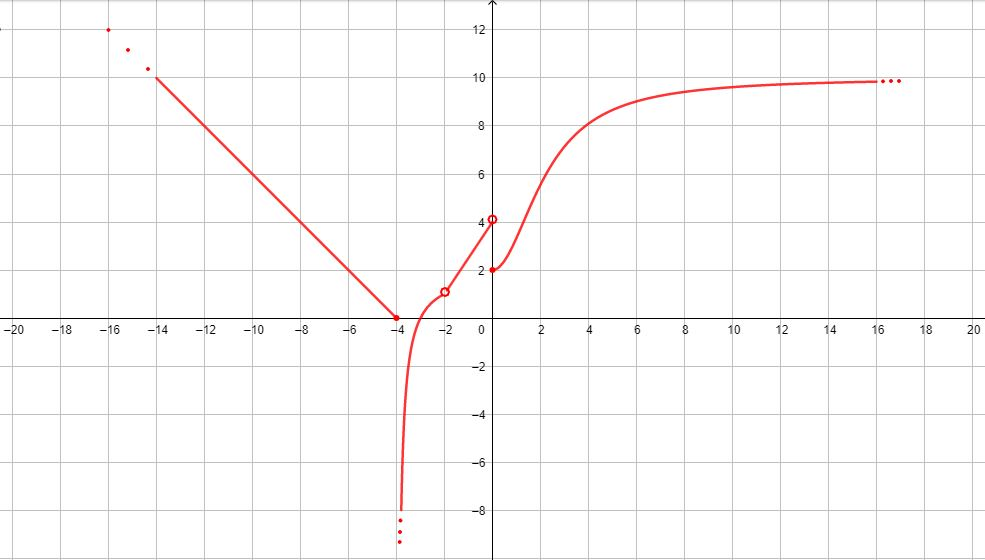
\includegraphics[scale=0.6]{solucion_2.png}
    \label{fig:solucion_2}
  \end{figure}
\end{soluciones}